%!TEX
% Author: Bhishan Poudel
\documentclass[12pt,A4]{article}
\usepackage[utf8]{inputenc}
\usepackage[english]{babel}
\usepackage{verbatim}
\usepackage{xspace} % For spacing
\usepackage{natbib} % For bib files
\usepackage{amsmath} % boldsymbol{} needs this.
\usepackage{mathrsfs} % For referencing math environment
\usepackage[usenames,dvipsnames,svgnames,table]{xcolor} % For colors
\usepackage{graphicx,subfigure} % For figures
\graphicspath{ {figures/}{../figures/} } % Put figures inside this directory and use pdf
\usepackage[parfill]{parskip} % to avoid indentation in paragraphs
\usepackage{enumitem} % for listing
\usepackage[ampersand]{easylist}
\ListProperties(Hide=100, Hang=true, Progressive=3ex, Style*=-- ,
Style2*=$\bullet$ ,Style3*=$\circ$ ,Style4*=\tiny$\blacksquare$ )    % for easylist
\usepackage{hyperref} % for hyper-link

% Math newcommands
\usepackage{mathtools}
\DeclarePairedDelimiter\abs{\lvert}{\rvert}
\DeclarePairedDelimiter\norm{\lVert}{\rVert}

\newcommand{\bvi}{\hat{\mathbf{i}}} %basis vector i
\newcommand{\bvj}{\hat{\mathbf{j}}} %basis vector j
\newcommand{\bvk}{\hat{\mathbf{k}}} %basis vector k
\newcommand{\bvr}{\hat{\mathbf{r}}} %basis vector r
\newcommand{\bvt}{\hat{\mathbf{\theta}}}%basis vector theta
\newcommand{\bvx}{\hat{\mathbf{x}}} %basis vector x
\newcommand{\bvy}{\hat{\mathbf{y}}}%basis vector y
\renewcommand{\v}[1]{\mathbf #1}%% $\v{a}$ gives bold a ).

%% My customized definitions
\usepackage{mydefs}
\newcommand{\vsn}[1]{(\textcolor{brown}{BP: #1})}
\newcommand{\dc}[1]{(\textcolor{magenta}{DC: #1})}

%%%%%%%%%%%%%%%
\begin{document}

% %%%%%%% cover-page
\thispagestyle{empty}
\begin{center}
\textbf{Effects of Wavelength Dependence on Galaxy Shear Measurement} \\

\vspace{2cm}
PH.D. THESIS PROSPECTUS BY BHISHAN POUDEL \\
(ADVISOR: ASSOCIATE PROF. DOUGLAS CLOWE) \\

\vspace{3cm}
\it{
Department of Physics and Astronomy\\
Ohio University\\
Athens, OH 45701\\
\vspace{2cm}
bp959314@ohio.edu\\
}


\vspace{3cm}
\it{
COMMITTEE MEMBERS\\}
\it{
Dr. XXX\, \hspace{3mm} (Department of Physics \& Astronomy)\\
Dr. XXX\, \hspace{3mm} (Department of Physics \& Astronomy)\\
Dr. XXX\, \hspace{3mm} (Department of Chemistry \& Biochemistry)
}

\end{center}
%
%
%#******************************************************************************
%#==============================================================================
%#          List of Acronyms
%#==============================================================================
%#******************************************************************************
%
\thispagestyle{empty}
\begin{center}
\textbf{ACRONYMS}
\end{center}
\textbf{CDM}    \hspace{9.5mm} Cold Dark Matter \\
\textbf{CMB}    \hspace{10mm} Cosmic Microwave Background \\
\textbf{DE}     \hspace{15mm} Dark Energy \\
\textbf{DM}     \hspace{14mm} Dark Matter \\
\textbf{FWHM}   \hspace{6mm} Full Width Half Maximum \\
\textbf{GR}     \hspace{15mm} General Relativity \\
\textbf{HST}    \hspace{13mm} Hubble Space Telescope \\
\textbf{IMCAT}  \hspace{7mm} Image and Catalog Manipulation Software \\
\textbf{LSS}    \hspace{15mm} Large Scale Structure \\
\textbf{LSST}   \hspace{12mm} Large Synoptic Survey Telescope \\
\textbf{PSF}    \hspace{14mm} Point Spread Function \\
\textbf{SED}    \hspace{14mm} Spectral Energy Distribution \\
\textbf{WFIRST} \hspace{4mm}  Wide-Field Infra-red Survey Telescope \\
\clearpage
%longest word wfirst is 6 letter long and make it 4mm wide.
%one letter less is about 3mm longer space.
%
%

%%%%%%%%%%% TOC
\clearpage
\tableofcontents
\listoffigures
\listoftables
\clearpage


% Rest of the chapters
\section{Introduction}\label{sec:intro}
Gravitational Lensing provides us a way to see how dark matter along with 
visible matter is distributed in universe. This theory of gravitational lensing is supported by Einstein's general theory of relativity which predicts the deflection of light in a gravitational field if any massive object is present there (\cite{hartle03}).
%
%
%```````````````````````````````````````````````````````````````````````````````
%         Subsection : Einstein's Deflection Angle
%```````````````````````````````````````````````````````````````````````````````
%
\subsection{Einstein's Deflection Angle}
  % aug 14, sch06  page 64
  \begin{figure}[ht!]
      \centering
      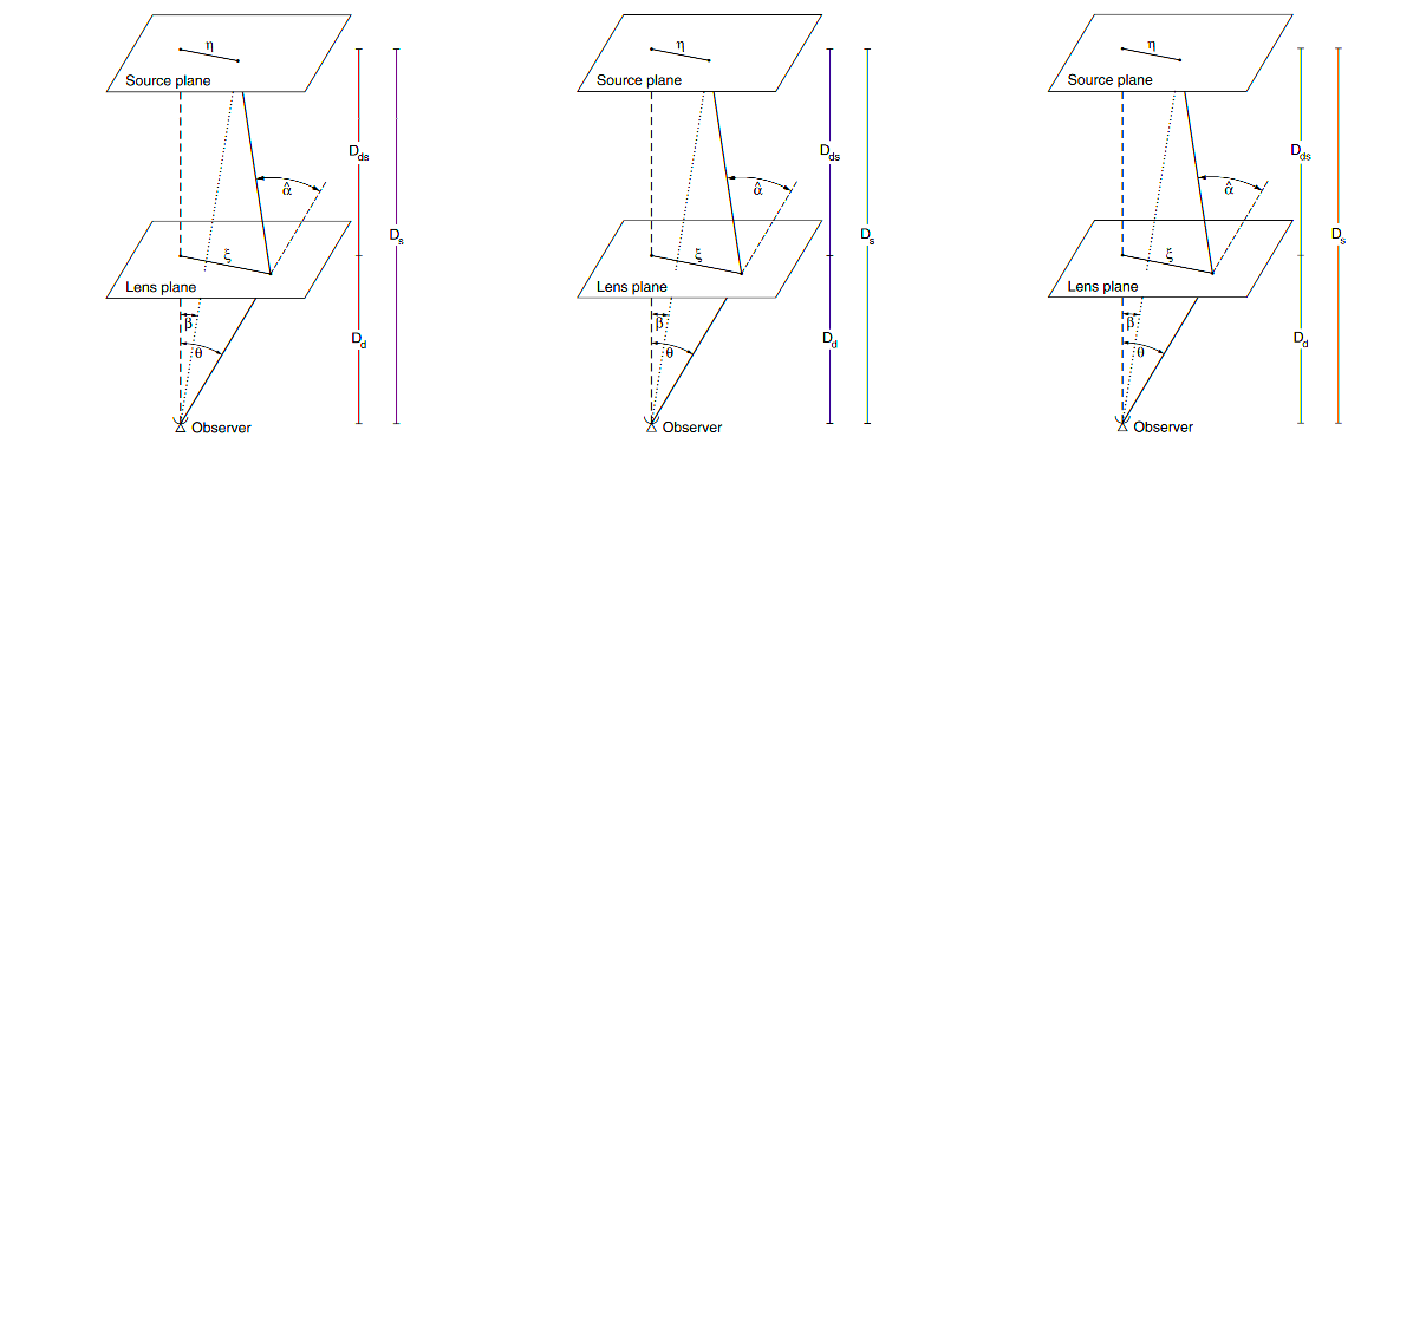
\includegraphics[width=0.5\textwidth]{grav_lensing}
      \caption[Simple sketch to gravitational lensing.] {Simple sketch to gravitational lensing ~\protect\cite{barSch_01}} %{~\protect\cite{barSch_01} } % \protect ~\cite{barSch_01}
      \label{[fig:lensing] }% \protect \cite{barSch_01}
  \end{figure} % (Bartelmann and Schneider 2001)}
  

  General Relativity predicts that when the beam of light passes through near
  the massive objects, the rays of light undergo deflection from their original path.
  This angle of deflection was predicted by Einstein's theory of General Relativity.
  According to this theory if the massive object of mass $M$ is located at a
  perpendicular distance $\xi$ (called \textbf{impact parameter}) from the line of sight
  of source and the observer then the deflection caused by that mass is given by
  \cite{sch07}
  \begin{equation}
    \hat{\alpha} = \frac{4GM}{c^2\xi}.
    \label{[eq:deflection]}
  \end{equation}

  This equation (\ref{[eq:deflection]} ) is valid only when the angle
  $\hat{\alpha} <<1  $ . In  case of gravitational lensing, the product of mass of the
  deflector and the Gravitational Constant is always the much smaller than the
  squared of velocity of light, thus making the deflection angle very small.

  For quantitative purpose,
  we can calculate the value of deflection angle for distant stars appearing near to the
  solar limb by setting the mass $M = M_{\odot}$ and radius $ R = R_{\odot}$ in the above equation to obtain the angle of deflection $\hat{\alpha} = 1.74''$. This value was tested
  in famous solar eclipse experiment in May 29, 1991 which was conceived by Sir Frank Watson Dyson, Astronomer Royal of Britain in 1917 and led by Sir Arthur Stanley Eddington
  two years later in 1919 (\cite{eclipse19}). The experiment was designed to test following hypotheses:



  \begin{itemize}

    \item{The light path is uninfluenced by gravitations.}
    \item{The law of gravitation will follow Newtonian law and will produce
            0''.87 apparent displacement}
    \item{The course of ray of light will follow Einsteins generalized
            relativity and lead to apparent displacement of 1.74''.}
  \end{itemize}
  The experiment concluded that the results were close to the Einsteins predicted
  deflection angle and thus supporting the gravitational lensing theory.

  %capranico 63 and schBar 327
  This was the deflection due to point source. We can also define the delfection
  for the extended mass with certain surface mass density $\Sigma$ as
  \begin{equation}\label{[eq:alphaHat]}
    \hat{\boldsymbol{\alpha}} (\boldsymbol{\xi} ) = \frac{4G}{c^2} \int d^2 \boldsymbol{\xi\prime}\quad  \Sigma (\boldsymbol{\xi\prime}) \quad  \frac{\boldsymbol{\xi} - \boldsymbol{\xi\prime}}{|\boldsymbol{\xi} - \boldsymbol{\xi\prime} |^2}
  \end{equation}
  Here, the \textit{surface mass density} $\boldsymbol{\Sigma}$ is defined as,
  \begin{equation}\label{[eq:surface_mass_density]}
    \boxed{
    \Sigma(\boldsymbol{\xi}) \equiv \int dr_3 \ \rho(\xi_1, \xi_2, r_3)} \quad (\text{Surface Mass Density})
  \end{equation}
  which is the mass density projected onto the lens plane, perpendicular to the
  light ray, and $r_3$ is the coordinate along the line of sight, and
  $\xi_1$, $\xi_2$ the other two perpendicular coordinates.


  %
  %
  %```````````````````````````````````````````````````````````````````````````````
  %         Subsubsection : Lens equation
  %```````````````````````````````````````````````````````````````````````````````
  %
\subsection{Lens equation}
  We consider a simplistic lensing model in which lens and the source objects are
  point objects. The observer observes the rays of light from the source at a
  distance $D_s$ which pass through the gravitational influence field of a massive
  object of mass M and distance $D_d$ located perpendicularly $\boldsymbol{\xi}$ distance away
  from line of sight (also called impact parameter).


  Let  $\boldsymbol{\eta}$  denotes the true, two-dimensional position of the
  source in the source plane and $\boldsymbol{\beta}$ is the true angular position
  of the source. This means in absence of light deflection we would have,
  \begin{equation}\label{[eq:beta]}
    \boldsymbol{\beta} = \frac{\boldsymbol{\eta} }{D_s}.
  \end{equation}
  The relation between position $\boldsymbol{\xi}$ and $\boldsymbol{\theta}$  is
  given by,
  \begin{equation}\label{[eq:theta]}
    \boldsymbol{\theta} = \frac{\boldsymbol{\xi} }{D_d}.
  \end{equation}
  This means $\boldsymbol{\theta}$ is the observed position of the source on the
  sphere relative to the position of center of the lens which is the origin of
  the coordinate system with $\boldsymbol{\xi} = 0$. Where, $D_{ds}$ is the distance of
  the source plane from the lens plane.


  Here we adopt the relation,
  \begin{equation}\label{[eq:D_ds]}
    D_{ds} = D_s - D_d.
  \end{equation}
  This relation holds true as long as the relevant distances are much smaller
  than the radius of the universe ($c/H_0$) and this is always the case for
  distances within our Galaxy and in Local Group. However, this relation no longer
  holds true for cosmological distances between source and lenses.

  From the figure (\ref{[fig:lensing]}), we can relate $\boldsymbol{\eta}$ with
  deflection angle $\boldsymbol{\alpha}$ as
  \begin{equation}\label{[eq:eta]}
    \boldsymbol{\eta} = \frac{D_s}{D_d} \boldsymbol{\xi} - D_{ds} \hat{\boldsymbol{\alpha} } (\boldsymbol{\xi} ).
  \end{equation}

  Using equation (\ref{[eq:beta]}) we can write $\boldsymbol{\beta}$ as
  \begin{equation}\label{[eq:beta2]}
    \boldsymbol{\beta} = \boldsymbol{\theta} - \frac{D_{ds}}{D_s}\  \hat{\boldsymbol{\alpha} } (D_d \boldsymbol{\theta} ).
  \end{equation}

  In this equation (\ref{[eq:beta2]}) we have some factor multiplying the
  deflection angle, so we define \textit{reduced deflection angle}
  \begin{equation}\label{[eq:alphaReduced]}
    \boxed{\boldsymbol{\alpha} (\boldsymbol{\theta} ) = \frac{D_{ds}}{D_s}\  \hat{\boldsymbol{\alpha}} (D_d \boldsymbol{\theta} )} \quad (\text{Reduced Deflection Angle})
  \end{equation}

  and then rewrite the lens equation (\ref{[eq:beta2]}) as
  \begin{equation}\label{[eq:beta3]}
     \boldsymbol{\beta} = \boldsymbol{\theta} - \boldsymbol{\alpha} (\boldsymbol{\theta} ).
  \end{equation}

  For a point mass object, using the equations (\ref{[eq:alphaHat]}) and (\ref{[eq:theta]}) the equation of reduced deflection angle (\ref{[eq:alphaReduced]})
  becomes
  \begin{equation}\label{[eq:alphaAbs]}
    \abs{\boldsymbol{\alpha} (\boldsymbol{\theta} )} = \frac{D_{ds}}{D_s}\  \frac{4GM}{c^2 D_d \abs{\boldsymbol{\theta}  }}.
  \end{equation}


%
%
%```````````````````````````````````````````````````````````````````````````````
%         Subsubsection : Convergence and Deflection Potential
%```````````````````````````````````````````````````````````````````````````````
% \texorpdfstring{$math$}{alternative} is to avoid Hyperref warning 
%                                      Token not allowed in a PDF string
\subsection{Convergence \texorpdfstring{$\kappa$ and deflection potential $\psi$}{kappaDefletionPotential}}
  % sch bar 328 Aug 22, 2017 Tue
  Then convergence is defined as the ratio of the surface mass density of the lens
  and the critical surface mass density as like

  \begin{equation}\label{[eq:kappa]}
    \boxed{\kappa (\boldsymbol{\theta} ) \equiv \frac{\Sigma (D_d \boldsymbol{\theta} )}{\Sigma_{cr}}} \quad (\text{Convergence}).
   \end{equation}
  Where, the critical surface mass density is given by
  \begin{equation}\label{[eq:crit_surf_mass_density]}
    \Sigma_{cr} = \frac{c^2}{4\pi G} \frac{D_s}{D_d D_{ds}}.
  \end{equation}
  The critical density depends on the redshift of source and lens.
  If the convergence $\kappa \geq 1$ i.e. surface density is less than critical
  surface density then we can see the multiple images of the source. If the
  value of $\kappa$ is very large it is called "strong gravitational lensing"
  and if it is only slightly greater than one, it is called "weak gravitational lensing".
  So, the value of critical mass density plays the role in distinguishing weak
  vs. strong gravitational lensing.

  Moreover, we can define scaled deflection angle in terms of convergence as
  \begin{equation}\label{[eq:alpah_kappa]}
    \boldsymbol{\alpha}(\boldsymbol{\theta} ) = \frac{1}{\pi}\ \int d^2 \theta\prime \ \kappa(\boldsymbol{\theta}\prime) \ \frac{\boldsymbol{\theta} - \boldsymbol{\theta\prime} }{\abs{\boldsymbol{\theta} - \boldsymbol{\theta\prime} }^2}\  .
  \end{equation}
  and the \textit{deflection potential} can be defined as
  \begin{equation}\label{[eq:psi]}
    \psi(\boldsymbol{\theta}) = \frac{1}{\pi}\  \int d^2 \theta\prime \ \kappa(\boldsymbol{\theta\prime} ) \ ln\abs{\boldsymbol{\theta} - \boldsymbol{\theta\prime}}.
  \end{equation}
  

%
%
%```````````````````````````````````````````````````````````````````````````````
%         Subsubsection : Multiple Images
%```````````````````````````````````````````````````````````````````````````````
%
\subsection{Multiple Images}
  We can see the multiple images of the source at different places
  $\boldsymbol{\theta}_i $ if the equation (\ref{[eq:beta3]})
  holds true for different values of the deflection angles.

  \begin{figure}[ht!]
      \centering
      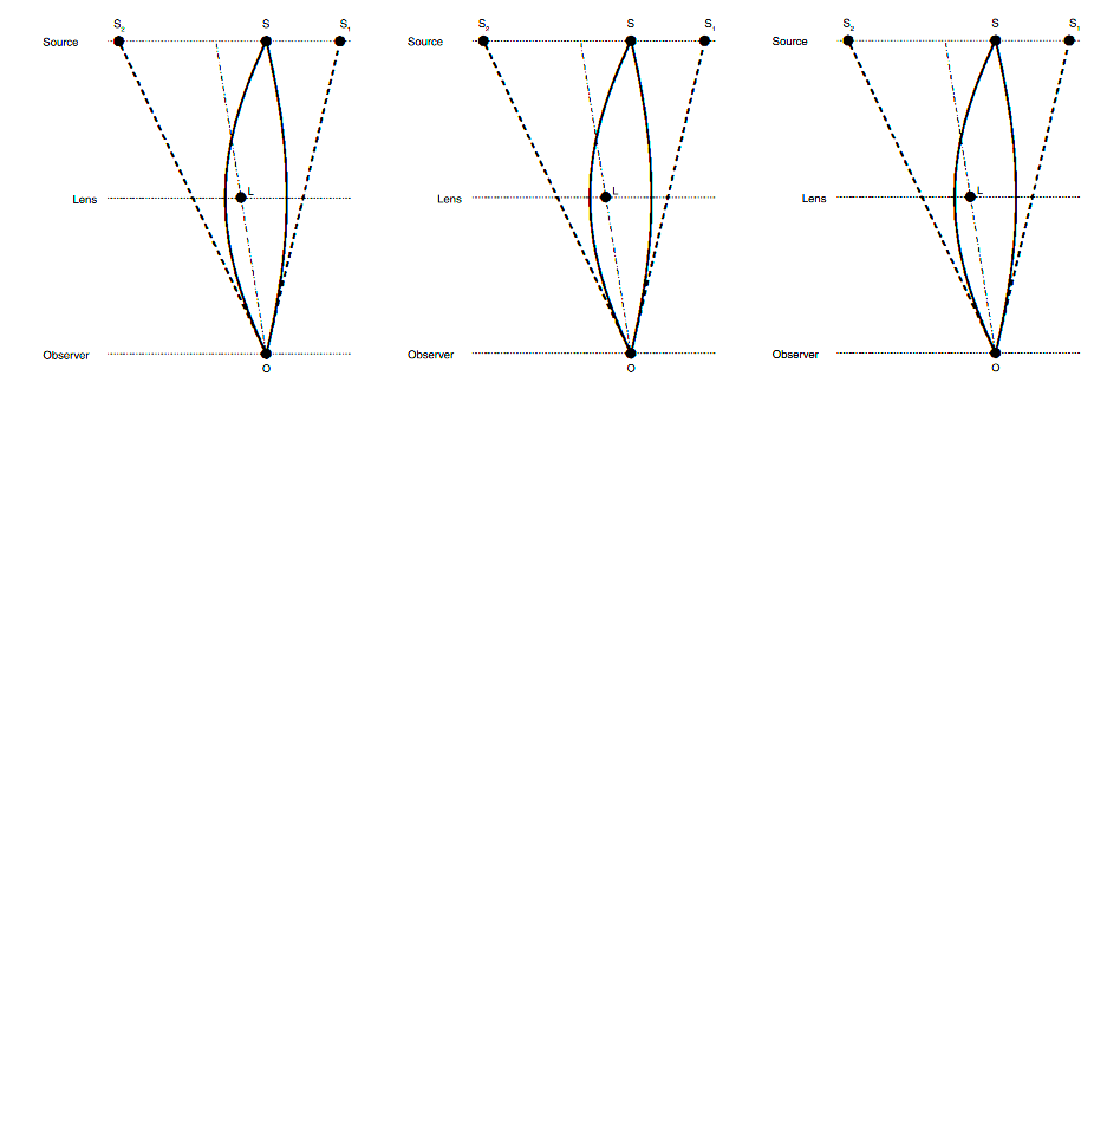
\includegraphics[width=0.5\textwidth]{multiple_images}
      \caption[Multiple images of single source]{Multiple images of single source ~\protect\cite{sch07}}
      \label{[fig:multiple_images]}
  \end{figure}

  This figure illustrates a typical situation in which there are two images $S_1$
  and $S_2$ of the single source $S$ which is lensed by the point massive object
  $L$.

  Here, if we take direction of deflection angle as pointing towards the source,
  we can write the deflection angle for the point mass (\ref{[eq:alphaAbs]}) as
  \begin{equation}\label{[eq:alpha_point_mass]}
    \boxed{\boldsymbol{\alpha} (\boldsymbol{\theta}  ) \equiv \frac{4GM}{c^2}\  \frac{D_{ds}}{D_s D_d}\  \frac{\boldsymbol{\theta} }{\abs{\boldsymbol{\theta}}^2}} \quad (\text{Reduced Deflection Angle})
  \end{equation}

  Now, we define \textit{Einstein angle} as
  \begin{equation}\label{[eq:einstein_angle]}
    \boxed{\theta_E = \sqrt{\frac{4GM}{c^2}\  \frac{D_{ds}}{D_s D_d}}} \quad (\text{Einstein Angle}).
  \end{equation}
  Then, we can rewrite the equation (\ref{[eq:alpha_point_mass]}) as
  \begin{equation}\label{[eq:beta_einstein]}
    \boldsymbol{\beta} = \boldsymbol{\theta} - {\theta_E}^2 \ \frac{\boldsymbol{\theta} }{\abs{\boldsymbol{\theta}  }^2 }
  \end{equation}

  To solve this equation (\ref{[eq:beta_einstein]}) we define two scaling factors
  \begin{equation}\label{[eq:x_y_lens]}
    y = \frac{\boldsymbol{\beta} }{\theta_E}\  ; \  x = \frac{\boldsymbol{\theta} }{\theta_E}
  \end{equation}

  Then we get
  \begin{equation}\label{[eq:y_lens]}
    \textbf{y} = \textbf{x} - \frac{\textbf{x}  }{\abs{\textbf{x}  }^2}.
  \end{equation}

  This is a quadratic equation and the solutions are given by,
  \begin{equation}\label{[eq:x_lens]}
    \textbf{x} = \frac{1}{2} (\abs{\textbf{y}} \pm \sqrt{4+ \abs{\textbf{y} }^2}) \
    \frac{\textbf{y} }{\abs{\textbf{y} }}.
  \end{equation}

  Following information can be drawn from the solution of lens equation:
  \begin{easylist}

    & {Except for the divergence condition $\theta \rightarrow 0$ any source at position $y$ has two images.}
    & {The two images are on the opposite sides of the source position when viewed from observer position.}
    & {If the source is exactly behind the lens ($\textbf{y} = 0$), we see the circular \textit{Einstein ring}. }
    & { \textit{Einstein ring} has the angular diameter $2 \theta_E $ and it gives the characteristic images separation.}
  \end{easylist}

  %
  %
  %```````````````````````````````````````````````````````````````````````````````
  %         Subsubsection : Magnification and Shear
  %```````````````````````````````````````````````````````````````````````````````
  %
\subsection{Magnification $\mu$ and shear $\gamma$ }
  The light rays in gravitational are not bent uniformly, the ones near to the
  lens are deviated more and the ones that are farther are bent in smaller
  proportion. This differential deflection gives rise to the distorted and
  magnified images of the source object.

  Let $\textbf{I}^s(\boldsymbol{\beta} )$  be the surface-brightness distribution
  of the source, then following the conservation of total surface brightness
  the observed surface-brightness distribution in the lens
  plane is given by
  \begin{equation}\label{[eq:I_theta]}
    \boldsymbol{I(\theta)} =  \textbf{I}^s \ [\boldsymbol{\beta}(\boldsymbol{\theta})].
  \end{equation}


  Now we expand the \textit{true angular position} of the source $\boldsymbol{\beta}$
  in terms of \textit{observed angular position} of the source $\boldsymbol{\theta}$
  using Taylor expansion around the central observed position $\boldsymbol{\theta_0}$
  we get

  \begin{eqnarray}\label{[eq:beta_taylor]}
    \boldsymbol{\beta}(\boldsymbol{\theta} ) = \boldsymbol{\beta}_0 + ( \boldsymbol{\theta} - \boldsymbol{\theta}_0 ) \frac{\partial\boldsymbol{\beta} }{\partial\boldsymbol{\theta}  }
  \end{eqnarray}

  Here, the term differential of $\boldsymbol{\beta}$ w.r.t. $\boldsymbol{\theta}$ is called \textit{distortion matrix}

  \begin{eqnarray}\label{[eq:dist_matrix]}
    \boxed{ \mathscr{A}(\boldsymbol{\theta} ) \equiv \frac{\partial \boldsymbol{\beta} }{ \partial \boldsymbol{\theta} }} \quad (\text{Distortion Matrix}).
  \end{eqnarray}

  Now we can write the observed surface brightness $\boldsymbol{I(\theta)}$ in terms of
  distortion matrix as
  \begin{eqnarray}\label{[eq:I_taylor]}
    \boxed{\boldsymbol{I}(\boldsymbol{\theta}) = \boldsymbol{I}^s[\beta_0 + \mathscr{A}(\boldsymbol{\theta}) (\theta - \theta_0 ) ]} \quad (\text{Observed Surface Brightness})
  \end{eqnarray}

  In terms of deflection potential $\psi$  \textit{Jacobian matrix} $\mathscr{A}$
  can be written as
  \begin{align}\label{[eq:jacobian]}
    \mathscr{A}(\boldsymbol{\theta} ) & = \frac{\partial \boldsymbol{\beta} }{ \partial \boldsymbol{\theta} } \\
      & = (\delta_{ij} - \frac{\partial^2 \psi(\boldsymbol{\theta})}{\partial \theta_i \partial \theta_j}) \nonumber \\
      & = {  \begin{pmatrix}
               1 - \psi{,11}  &-\psi_{,12}  \\
               -\psi{,21}  & 1 - \psi_{,22} \ .
            \end{pmatrix}
          }
  \end{align}

  From these deflection potential terms, we define shear components
  \begin{eqnarray}\label{[eq:shear_comps]}
    \gamma_1 &=& \frac{1}{2} (\psi_{,11} + \psi_{,22} ) \\
    \gamma_2 &=& \psi_{,12}
  \end{eqnarray}

  Here, the two components tensor $\gamma$ is called \textit{shear} and is
  given by
  \begin{eqnarray}\label{[eq:shear]}
    \boxed{\gamma \equiv \gamma_1 + i \gamma_2
           = \lvert\gamma\rvert e^{2i \phi}} \quad (\text{Shear})
  \end{eqnarray}

  Here, $\gamma_1$ and $\gamma_2$ are two components of shear as given in equation
  (\ref{[eq:shear_comps]}) and $\phi$ is the phase angle.

  The shear has two components $\gamma_1$ and $\gamma_1$ which can be expressed as
  \begin{equation}\label{[eq:shear]}
    \gamma \equiv \gamma_1 + i \gamma_2 = \lvert\gamma\rvert e^{2i \phi}.
  \end{equation}
  Also, in terms of deflection potential the shear components can be expressed as
  \begin{eqnarray}\label{[eq:shear_comp]}
    \gamma_1 &=& \frac{1}{2} (\psi_{,11} - \psi_{,22} ) \\
    \gamma_2 &=& \psi_{,12} \nonumber
  \end{eqnarray}

  Also, the convergence $\kappa$ is related to the deflection potential through
  Poisson equation
  \begin{eqnarray}\label{[eq:kappa_psi]}
    \nabla^2 \psi(\theta) = 2 \kappa(\theta).
  \end{eqnarray}

  In terms of matrix elements of deflection potential $\psi$ we can write $\kappa$ as
  \begin{eqnarray}\label{[eq:kappa_psi]}
    \boxed{\kappa = \frac{1}{2} (\psi_{,11} + \psi_{,22})} \quad (\text{Convergence})
  \end{eqnarray}

  Now we can write the distortion matrix $\mathscr{A}$ in terms of
  shear components $\gamma_1$ and $\gamma_2$ and convergence $\kappa$ as
  \begin{eqnarray}\label{[eq:A_theta]}
    \mathscr{A}(\boldsymbol{\theta}) =
    \begin{pmatrix}
      1 - \kappa - \gamma_1 & - \gamma_2  \\
      - \gamma_2 & 1 - \kappa + \gamma_1
    \end{pmatrix}
  \end{eqnarray}

  If we solve this matrix we get the eigenvalues
  \begin{eqnarray}\label{[eq:eigen]}
    eig(\mathscr{A}) = 1 - \kappa \pm \lvert g \rvert .
  \end{eqnarray}

  The equation \ref{[eq:I_taylor]} has the shape of an ellipse. This means that
  if a circular galaxy is lensed then the resulting observed image will be an
  ellipse. The semi-major and semi-minor axes of the ellipse are given by
  \begin{eqnarray}\label{[eq:semi_axes]}
    a &=& \frac{R}{1 - \kappa  - \lvert g \rvert } \\
    b &=& \frac{R}{1 - \kappa  + \lvert g \rvert }
  \end{eqnarray}

  Here, $R$ is the radius of circular source, $a$ is the semi-major axis, $b$ is semi-minor axis, and $g$ is the reduced shear
  defined as
  \begin{eqnarray}\label{[eq:g]}
    \boxed{g(\boldsymbol{\theta} ) \equiv \frac{\gamma(\boldsymbol{\theta} )}{1 - \kappa(\boldsymbol{\theta} )}} \quad (\text{Reduced Shear}).
  \end{eqnarray}

  The inverse of the determinant of the matrix $\mathscr{\alpha}$ gives the
  magnification tensor. Then we define magnification as
  \begin{eqnarray}\label{[eq:magnification]}
    \boxed{\mu(\boldsymbol{\theta}) \equiv \frac{1}{det \lvert \mathscr{A} \rvert }} \quad (\text{Magnification}).
  \end{eqnarray}
% Author: Bhishan Poudel
% Dates I worked:
%  Nov 2, 2017
%
%
%#*******************************************************
%#=======================================================
%# Chapter 2: Galaxy Fitting
%#=======================================================
%#*******************************************************
%
%
\section{Galaxy Fitting}\label{sec:chap2}
In this section, we want to fit the bulge and disk component fitting to the base 
galaxy images provided from HST survey. We use the software called 
\textit{Galfit} \footnote{https://users.obs.carnegiescience.edu/peng/work/galfit/galfit.html}
to get the reasonable components of the base galaxy. Galfit is an image analysis
algorithm that can model profiles of any given astronomical objects in the given
fits image of the data sample. For example, if an fits image contains a galaxy,
we can use galfit to fit the bulge and disk components to that galaxy.

Here, for the bulge part of the galaxy, we use the de Vaucouleurs profile in 
Galfit.
The de Vaucouleurs profile describes how the surface brightness of a giant
elliptical galaxy changes as a  function of the radius R from the center of the
galaxy.

Let $R_e$ be the radius of an isophote containing the half of the total 
luminosity for a galaxy, then, for a de Voucouleurs profile, the surface 
brightness enclosed by the radius $R$ in that galaxy is given by:

\begin{eqnarray}\label{[eq:devauc]}
    I(R) = I_e e^{-7.669 [ (R/R_e)^{1/4} -1]  }
\end{eqnarray}

Galfit has this formula as a built-in feature to get the bulge component of the
galaxy.

Similarly, to fit the disk profile to a galaxy, we use the profile called 
\textit{exponential disk profile} in Galfit. This exponential disk profile 
is a special case of Sersic profile. In the Sersic
profile, the total surface brightness enclosed by the radius R around the center
of a galaxy is given by

\begin{eqnarray}\label{[eq:sersic]}
    ln \ I(R) = ln \ I_0 - k R^{1/n}
\end{eqnarray}

where, $I_0$ is the central surface brightness at $R = 0$ and the parameter n is 
called \textit{Sersic index} which determines the curviness of the Sersic profile.

For the most of the spiral galaxies and dwarf elliptical galaxies, the Sersic index
is close to 1. This case when the Sersic index n is equal to 1 is called
exponential disk profile.
In exponential disk profile, the surface brightness inside the radius R is given
by

\begin{eqnarray}\label{[eq:expdisk]}
    ln \ I(R) = ln \ I_0 - k R
\end{eqnarray}

In this project we have 201 base galaxies obtained from the HST survey. As we 
know that some of the galaxies have both bulge and disk components and some
do not have it. For the case, when the base galaxy has bulge-disk components,
Galfit gives nice bulge and disk components, however, when the base galaxy itself
does not have reasonable bulge-disk component, Galfit can not give bulge and disk
components of that galaxy. In that case either Galfit fails to give two 
components or, gives bad parameter. We can see the whether the fitted parameters
are good or bad in the log file created from the Galfit. If a parameter is 
enclosed by \* then, we can not trust the fitting, and we treat like the given
galaxy does not have reasonable bulge-disk components.

Let's say we get two successful bulge and disk components of
a base galaxy, then we choose devauc profile as the bulge and exponential profile
as the disk image. On the other hand, if either the Galfit fails to produce
two component fittings or gives non-reliable fitting parameters, then we make some 
assumptions how to choose bugle and disk components. 
If the single component fitting of \textit{devauc profile} gives the better fit 
parameters than single component fitting of \textit{expdisk profile} ,
we choose the base galaxy as the bulge component and we
choose an empty image as the disk component. 
Similarly, if the single component \textit{expdisk profile} gives better fitting than 
single component \textit{devauc} fitting, we choose the base galaxy as the disk component 
and we choose an empty image as the bulge component. We may notice that,
while doing the galaxy fitting to our 201 base galaxies, we found that most the galaxies
gave better fit for the \textit{devauc profile} than the \textit{expdisk profile}.
An example of input parameter file for \textit{Galfit} is shown next page.
\newpage

\verbatiminput{sections/expdisk_devauc.sh}


Another point to note is that, to use the Galfit program, we need to use a PSF image
to convolve the original galaxy with the given PSF. The PSF image is different for 
different filter images of a given galaxy. That is, for F814W filter of a base
galaxy $galaxy\_f814w0.fits$ we use the psf $psf\_f814w.fits$ and for the galaxy
$galaxy\_f660w0.fits$ we use the psf $psf\_f606w.fits$. For all the F814W filter
images we use the same $psf\_f814w.fits$ and for all the F606W filter images we use
the same $psf\_f066w.fits$.

Here, in our project we use the F814W filter images taken from the HST ACS Wide Field Channel Camera.
To create the relevant PSF, we use an on-line tool called  \textit{STScI TinyTim Web Application} 
\footnote{http://www.stsci.edu/hst/observatory/focus/TinyTim}.

The TinyTim web application needs some parameters to create a psf.
For this project we chose the following parameters:

\begin{table}[!h]
\centering
\caption{Tiny Tim Parameters}
\label{tiny-tim}
\begin{tabular}{ll}
Camera         & ACS - Wide Field Channel \\
Chip           & 1                        \\
Pixel Position & 301 301                  \\
Filter         & F814w                    \\
Spectrumtype   & Blackbody                \\
Spectrumvalue  & 6000                     \\
PSF diameter   & 5.0 arcsec               \\
Focus          & 0.0                     
\end{tabular}
\end{table}


% Author: Bhishan Poudel
% Date  :
% Update:
%
%
%#*******************************************************
%#=======================================================
%# Chapter 3: PSF Creation Using PhoSim
%#=======================================================
%#*******************************************************
%
%
\section{Chapter 3: PSF Creation Using PhoSim}\label{sec:chap3}
In case of galaxy fitting software \textbf{Galfit}, we created the PSF needed using an on-line tool called \textbf{TinyTim}. The PSF was specially designed for HST ACS Wide Field Camera observations. Here, we again want to create a general purpose PSF using a flat SED. SED stands for "Spectral Energy Distribution" which is simply a table of flux and wavelength. In our galaxy simulation program \textbf{Jedisim}, we use the PSF created by a program called '\textbf{PhoSim}'. PhoSim is a photon simulator application which uses Monte Carlo codes to calculate the physics of the atmosphere and the telescope \& camera optics. \footnote{$https://bitbucket.org/phosim/phosim_release/wiki/Home$}

To run \textbf{PhoSim}, we need a SED file, an instance catalog and a background file. Here, we are using flat SED file provided from SEDs list recommended from \textbf{PhoSim} website.
The plot of wavelength versus flux of flat sed is given below:
  \begin{figure}[ht!]
      \centering
      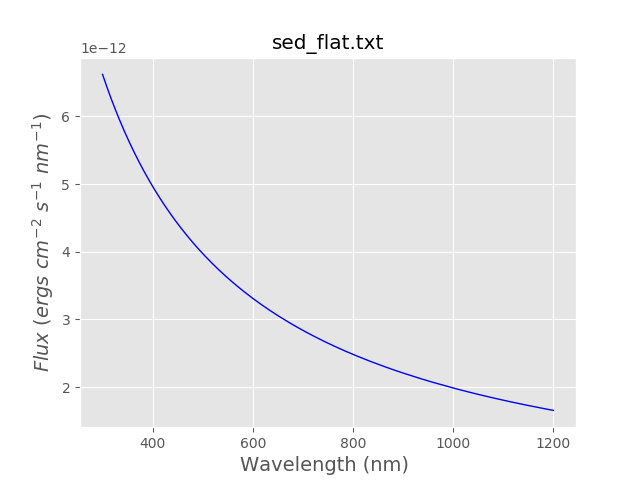
\includegraphics[width=0.5\textwidth]{sed_flat}
      \caption{Flat SED}
      \label{[fig:sed_flat]}
  \end{figure}

Here, the SED has flux values for wavelengths 400 to 1200 nanometers.
We are particularly interested only for the wavelength range of LSST r band filter. Looking at the file $phosim/data/lsst/filter\_2.txt$ and choosing only the range of the filter for transmission $>=5\%$ we get the range of 531 nm to 696 nm. From now on the range 531 nm to 696 nm will be called the
broadband range. We split this broadband into 21 equal parts and call each part a narrowband. For example, narrowband0 is from wavelength 5310 Angstrom to 5388 Angstrom. From these wavelengths we create 21 narrowband SED files and one broadband sed file. To get the psf using PHOSIM, we need three things: a sed file,an instance catalog, and a background file. We have got sed file from SEDs directory recommended by PhoSim, now we need to choose the background. For the background we chose a simple background file as shown below: 
\verbatiminput{seds/background1.txt}

 The third component needed is instance catalog file. The important parameters in an instance catalog are SIM\_SEED, SIM\_VISTIME, and object.
 The output PSF file will depend on the initial random seed to the PhoSim software. For the simplicity, we choose this seed number to be 1000. Similarly we choose the simulation time to be 5 minutes (equal to 300 seconds) as the SIM\_VISTIME parameter.
The "object" parameter consist of multiple fields. For example, we have used:
\begin{verbatim}
object 0 0.0 0.0 24 ../../../Research/psf_creation_phosim/scripts/
narrowband_seds/narrowband0.sed 0 0 0 0 0 0 star none none

These fields corresponds to following settings:
object ID RA DEC MAG_NORM SED_NAME REDSHIFT GAMMA1 GAMMA2 KAPPA DELTA_RA DELTA_DEC SOURCE_TYPE source_pars DUST_REST_NAME dust_pars_1 DUST_LAB_NAME dust_pars_1

The non-trivial components are magnitude of the star, name of the sed file used and source type (here, it is star).
\end{verbatim}
\footnote{https://bitbucket.org/phosim/phosim\_release/wiki/Instance\%20Catalog}
An example of instance catalog file can be found in PhoSim software
installation directory $phosim/examples/small\_catalog$.
An example of the instance catalog we used is given below: 
\verbatiminput{seds/narrowband0.txt}

The PHOSIM gives multiple outputs, out of which what we are interested in only the electron image named as $lsst\_e\_99999999\_f2\_R22\_S11\_E000.fits.gz$. For a given SED, we unzip this file and take as the psf file. Here for the broadband sed we got our psf for the broadband settings. However, the program \textbf{Jedisim} needs 21 narrowband psf images. To get these 21 narrowband psf images, we feed the 21 narrowband sed files to the PhoSim and get the required psf images. We take the middle narrowband psf i.e. psf10.fits as the monochromatic psf. We also normalize the total flux across all the psf images. This means, we first calculate the total flux of psf10.fits and scale the flux of all other psf images.


% Author: Bhishan Poudel
% Date  : Jan 17, 2018
% Update:
%
%
%#*******************************************************
%#=======================================================
%#  Chapter 4: Galaxy Simulation
%#=======================================================
%#*******************************************************
%
%
\section{Chapter 4: Galaxy Simulation With Jedisim}\label{sec:chap4}
We want to create the realistic simulation of the LSST observation from the existing data from the
HST data. From chapter 2 we have created the bulge and disk component of the HST ACS Wide Filed Camera observations
of certain patch of the sky. 

\subsection{Creation of Scaled Bulge, Disk, and Monochromatic Images}
We have total 201 number of HST images, so we have 201 bulge images and 201 disk images.
From these two folders we create so called scaled\_bulge, scaled\_disk, and scaled\_bulge\_disk folders. For this,
we first find the bulge\_factor (bf) and disk\_factor (df) then we create scaled galaxies.

 \begin{eqnarray}
 scaled\_bulge = bf * bulge.fits \\
 scaled\_disk = df * disk.fits
 \end{eqnarray}
 
 

To find bulge and disk factors, first we find fraction for bulge ratio and fraction of disk ratio as follows:

 \begin{eqnarray}
 f_{ratb} = \frac{\int_{\lambda0}^{\lambda20} f_{bz}(\lambda)d\lambda}
 {\int_{\lambda{hst0}}^{\lambda_{hst20}} f_{bzcut}(\lambda)d\lambda} \\
 f_{ratd} = \frac{\int_{\lambda0}^{\lambda20} f_{dz}(\lambda)d\lambda}
 {\int_{\lambda{hst0}}^{\lambda_{hst20}} f_{dzcut}(\lambda)d\lambda}
 \end{eqnarray}
Here, $f_{bz}$ is the flux column from the SED file according the redshift $z$ for the bulge and $f_{bzcut}$ is the 
flux column for cutout galaxy. Here, we have used the galaxy cutout redshift as $ z_{cutout} = 0.2$. Similarly we have the flux columns for disk galaxies.

The wavelengths $\lambda_0$ and $\lambda_{20}$ are the LSST R-band filter blue and red wavelengths. This range is $5520 \AA$ to $6910 \AA$ (Refer to: $https://www.lsst.org/about/camera/features$).
We divide these wavelengths by a factor ($1 + z$) to get the range 2208 to 2764 for the redshift of 1.5.

Similarly, for the HST the wavelengths are $\lambda_{hst0} = 7077.5 \AA$ and $\lambda_{hst0} = 9588.5 \AA$ after dividing by $ 1 + z = 1.2$ we get $\lambda_{hst0} = 5897.9 \AA$ and $\lambda_{hst0} = 7990.4 \AA$. We can get more details about HST ACS/WFC filter at the website $http://www.stsci.edu/hst/acs/documents/handbooks/current/c05_imaging2.html$.

Then, we get bulge factor and disk factor using the formula:
 \begin{eqnarray}
 bf = \frac{F_b + F_d} {F_b * f_{ratb} + F_d * f_{ratd}} * f_{ratb} \\
 bd = \frac{F_b + F_d} {F_b * f_{ratb} + F_d * f_{ratd}} * f_{ratd} \\
 \end{eqnarray}
 
 where, $F_b$ is the flux of a bulge file (e.g. $simdatabase/bulge_f8/f814w_bulge0.fits$) and $F_d$ is the flux of a disk file (e.g. $simdatabase/disk_f8/f814w_disk0.fits$) for 201 bulge and disk files we have 201 bulge and disk factors.
 
After we get these bulge and disk factors we simply multiply them by the bulge.fits and disk.fits to get scaled\_bulge.fits and scaled\_disk.fits.

\subsection{PSF Creation for Bulge, Disk, and Monochromatic Images}
From the PHOSIM Software we have created 21 narrowband PSFs. Now we will use them to create PSF for scaled bulge, disk, and monochromatic images. The scaled psf files are given by formula:
\begin{eqnarray}
p_b = \frac{b0*p0 + b1*p1 + ... + b20*p20}{b0 + b1 + ... + b20} \\
p_d = \frac{d0*p0 + d1*p1 + ... + d20*p20}{d0 + d1 + ... + d20} \\
p_m = f_{rd} \ p_d + f_{rb} \ p_b
\end{eqnarray}
Here, $p_b$, $p_d$,and $p_m$ are psf for bulge, disk, and monochromatic respectively. Also the quantities $b0, b1, ..., b20$ and $d0, d1, ..., d20$ are bulge and disk weights for 21 narrowbands. These quantities are the integrated flux in the given narrowbands. For example, for LSST R band filter the blue and red wavelength range is 2208 to 2764 Angstrom. We divide this range into 21 parts and integrate the flux in that range to get the bulge and disk factor for that range using SED file for bulge and disk.

\subsection{Jedisim Simulations}
Jedisim is a computer simulator that simulates realistic LSST images from HST images using various physics parameters.
It was initially developed by Dr. Ian Dell'Antonio of Brown University (2014) and after that heavily expanded and maintained by Bhishan Poudel of Ohio University (2014-2018) with the help of Dr. Doug Clowe. 
This program takes in scaled bulge and scaled disk galaxies and finally will create chromatic and monochromatic lsst images. It will also create 90 degree rotated images for the chromatic and monochromatic lsst images.
The \textbf{Jedisim} program itself consist of various sub programs, which I will describe briefly below.

\subsubsection{Create the Catalogs for Jedisim}
We use the subprogram \textbf{jedicatalog} to create the three catalog files need by Jedisim. The files are \textbf{catalog.txt}, \textbf{convolvedlist.txt}, and \textbf{distortedlist.txt}. The \textbf{catalog.txt} file contains various important quantities of a galaxy. Each row of catalog.txt file contains following parameters: galaxy\_name, center\_x, center\_y, angle, redshift, pixscale, old\_magnitude, old\_radius, new\_magnitude, new\_radius, stamp\_name, distorted\_file\_name. We will need these parameters to transform the galaxies.

In the jedicatalog program we specify a galaxy by six parameters magnitude, radius, image, redshift,position, and angle.

\begin{description}
\item[Magnitude]
In this simulation we have chosen the simulated galaxies magnitudes within range $22 \le M \le 28$. The galaxies are distributed with the power law,
\begin{equation}
  P(M+dM) \propto 10^{BM}
  \label{eq:mag_power_law}
\end{equation}
    where $M$ is the magnitude and $B = 0.33\ln 10$ is an empirical constant (refer to \cite{benitez_04}). The magnitude zero-point is taken to be 30 throughout the simulations by convention

\item[Radius] The simulated galaxies have the magnitudes between 22 and 28. For each magnitudes, we have a radius database for r50 radii. We choose a radius randomly from that radius bin for the given magnitude.

\item[Image] The postage stamp image is chosen randomly from the list of r50 radii such that the chosen r50 radius
is larger than the radius of original galaxy. This makes 
sure that images are always sized down and no information is artificially created by scaling.

\item[Redshift] In this simulation we have chosen the fixed redshift of 1.5. However, we can choose random redshifts for each magnitude bin from magnitude 22 to 28 is we opt to vary the redshifts of galaxies. The redshift database was obtained from ZCOSMOS database.

\item[Position] The position of center of the postage stamps are chosen randomly 
from the range [301,40,660] . This range is taken to ensure that all 600 by 600
postage stamps lie completely within the range [0,40,960]. In later simulation step, we will trim the border by 480 pixels so as to ensure uniform distribution
of galaxies with typical edge effects.

\item[Angle] We chose the angle of orientation of a galaxy randomly between 0 to 360 degrees. We should note that the orientation of galaxies has three degree of
freedom, but since we are dealing with 2D projections of galaxies, we can only make the orientation random in one degree of freedom.

\end{description}
The \textbf{convolvedlist.txt} contains the names of files to be written after we convolve a galaxy with a psf. A typical row of
convolvedlist appears like this $jedisim\_out/out0/convolved/convolved\_band\_0.fits$. When we convolve a large fitsfile with a psf, due to the memory restrictions of computer instead of creating single large convolved file we create 6 convolved bands and later combine them into a single large convolved galaxy.

The \textbf{distortedlist.txt} contains the names of the galaxies that will be after we distort them using Singular Isothermal Profile Lens. A typical row of convolvedlist appears like this $jedisim\_out/out0/distorted\_0/distorted\_0.fits$. There are 12,420 rows and the last row is $jedisim\_out/out0/distorted\_0/distorted\_12419.fits$.

The program \textbf{jedicatalog} will create

\subsubsection{Transform the Galaxies}
We transform the scaled bulge, scaled disk, and scaled bulge\_disk files using \textbf{jeditransform}. This sub routine reads in the catalog file and various transforming physics parameters from that file and then transforms the galaxies. This program reads 201 bulge (or disk) galaxies and create 12,420 HST stamps.

\subsubsection{Distort the Galaxies}
Here, we use the Singular Isothermal Sphere (SIS) profile to 
lens the galaxies. We have chosen fixed position of the lens
to be (6144,6144) and taken dispersion velocity $\sigma_v = 1000 km/s$. In the singular isothermal profile the density is 
calculated as
\begin{equation}
\rho(r,\sigma_v) = \frac{\sigma_v^2}{2\pi Gr^2}
\end{equation}
where, G is the gravitational constant and r is radius in pixels. Since the total mass inside radius r diverges as r reaches to infinity, the SIS model is non-physical. However, when the profile is finitely bounded, it constitutes a possible physical distribution and can be used as a lens.

We may also use the Navarro-Frenk-White (NFW) profile which does
not suffer from the divergence problem. The NFW profile is 
given by:
\begin{equation}
\rho(r,\rho_0,R_s) = \frac{\rho_0}{\frac{r}{R_s} (1 + \frac{r}{R_s})^2}
\end{equation}
where, $\rho_0, and\ R_s$ are the parameters dependent on the halo we use.

\subsubsection{Convolve the Galaxies with the PSF}
After we distort the galaxies, we convolve the big HST image with the PSF. For the bulge components we convolve the big HST galaxy with scaled bulge psf and for the disk components we convolve the big HST image with scaled disk psf.

\subsubsection{Rescale the Galaxies from HST to LSST}
Until now, we have been dealing with the HST images and HST psf images. Now, we scale down the pixels of HST to LSST using a routine \textbf{jedirescale}. After rescaling we go to the PIXSCALE 0.2 of LSST from the PIXSCALE of 0.06 of HST.

For bulge components, the output of jedirescale gives us lsst\_bulge file and similarly disk components gives us lsst\_disk fits files. Also, for the bulge\_disk files we get lsst\_monochromatic unnoised file.

\subsubsection{Create Monochromatic LSST Image}
From the \textbf{jedirescale} program if we feed the bulge\_disk images as the input fits-files, we will get the lsst\_bulge\_disk fits-file as the output. We add the Poisson noise of mean noise 10 pixels to get the LSST monochromatic image.
This is one of the main output of the \textbf{Jedisim} program.

\subsubsection{Create Chromatic LSST Image}
From the \textbf{jedirescale} program we get lsst\_bulge and lsst\_disk images. We combine them and add the Poisson noise of mean noise 10 pixels to get the LSST chromatic image.
This is one of the main output of the \textbf{Jedisim} program.

\subsection{Rotated galaxies output from Jedisim}
If we run the \textbf{Jedisim} program for the normal case we will get two main outputs, namely, lsst.fits and lsst\_mono.fits. But, the galaxies are randomly orientated in the 
universe and we may also want the 90 degree rotated versions of the galaxies. For, this purpose, the program Jedisim, will also gives us 90 degree rotated versions of the output files named as lsst90.fits and lsst\_mono90.fits. So, in the end of one run of Jedisim we will get four important output files, two for non-rotated galaxies and two for rotated galaxies.
% Author: Bhishan Poudel
% Date  : Mar 2, 2018
% Update:
%
%
%#*******************************************************
%#=======================================================
%# Chapter 5: Shear Analysis
%#=======================================================
%#*******************************************************
%
%
\section{Chapter 5: Shear Analysis}\label{sec:chap5}
From the galaxy simulation program \textbf{Jedisim}, we get monochromatic and chromatic LSST simulated galaxies. We intend to
analyze the shear of these galaxies. For the shear analysis I use a program called \textbf{imcat}\footnote{https://www.ifa.hawaii.edu/~kaiser/imcat/}. First we create the parameter file for the psf called 'psf.par'. Then we create the lc catalog files for all of the chromatic and monochromatic files. From 1000 simulations files of chromatic and monochromatic files we get 1000 catalog files. We combine them and do some galaxy cutting, for example: 'rg > 2.9' and so on. After that we use the imcat command `etprofile` to get the ellipticities and shears. For the simulations we used redshift z = 0.7, F814W filter HST images. The results are given below:
\begin{figure}[ht!]
    \centering
    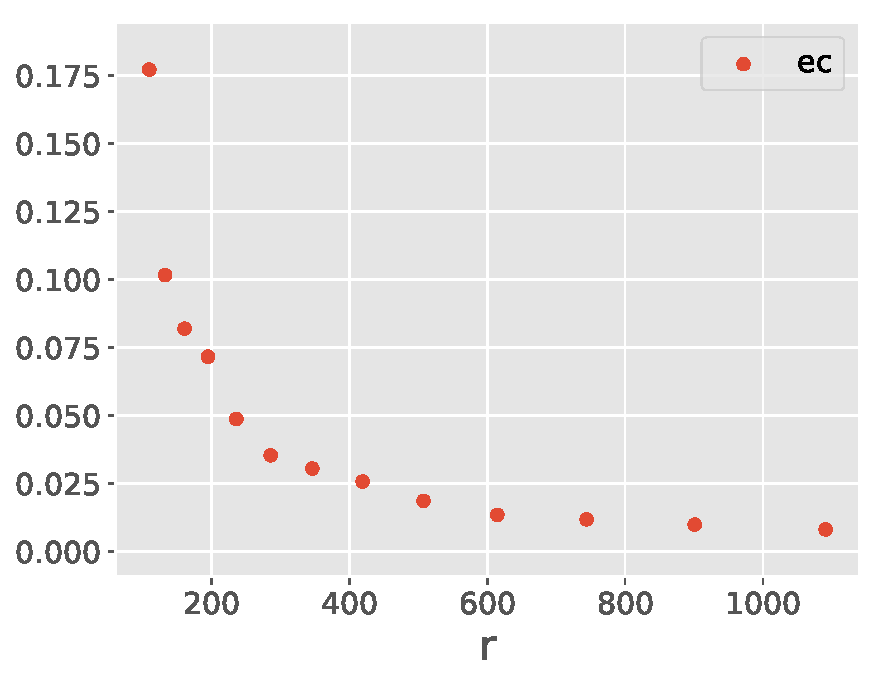
\includegraphics[width=0.48\textwidth,height=0.6\textwidth]{ec}
    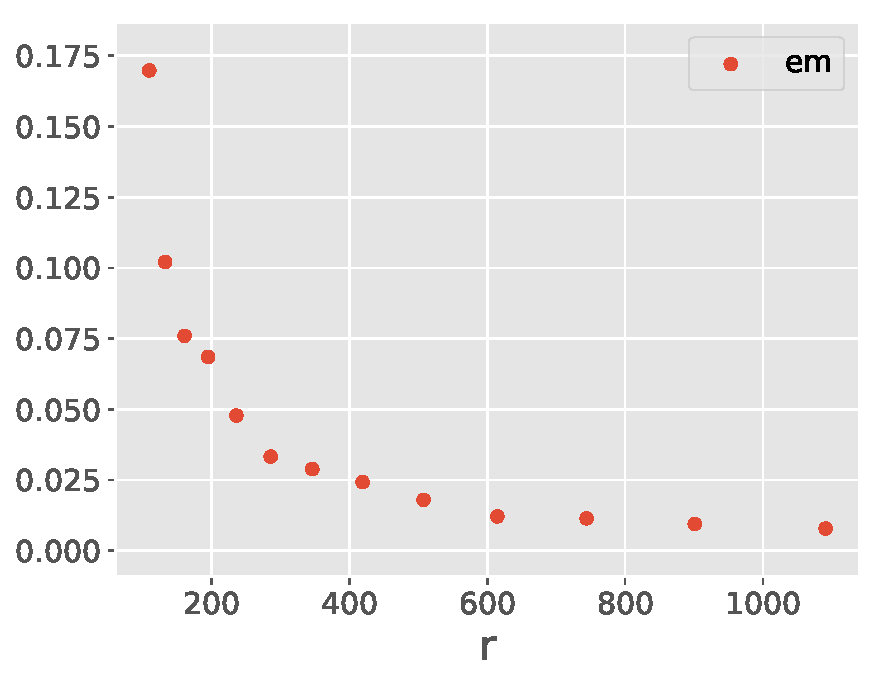
\includegraphics[width=0.48\textwidth,height=0.6\textwidth]{em}
    \caption{Ellipticites for chromatic and monochromatic files}
\end{figure}

\newpage
\begin{figure}[ht!]
    \centering
    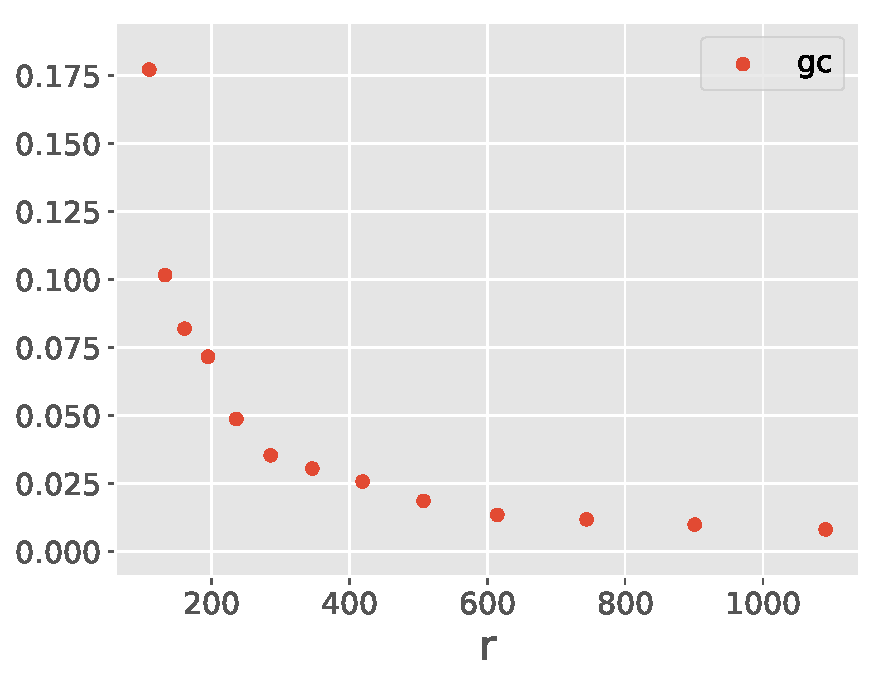
\includegraphics[width=0.48\textwidth,height=0.5\textwidth]{gc}
    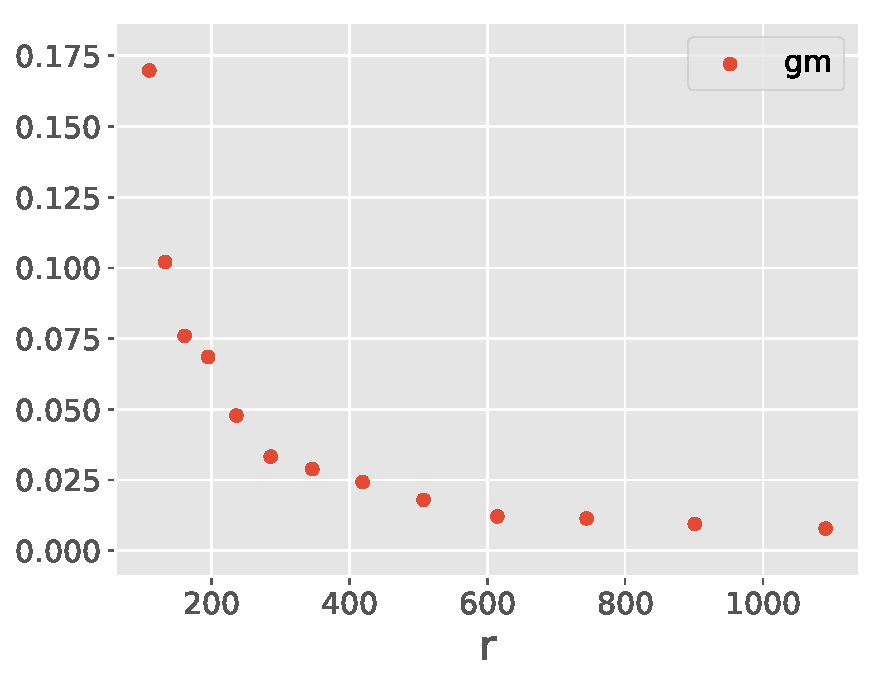
\includegraphics[width=0.48\textwidth,height=0.5\textwidth]{gm}
    \caption{Shears for chromatic and monochromatic files}
\end{figure}

\begin{figure}[ht!]
    \centering
    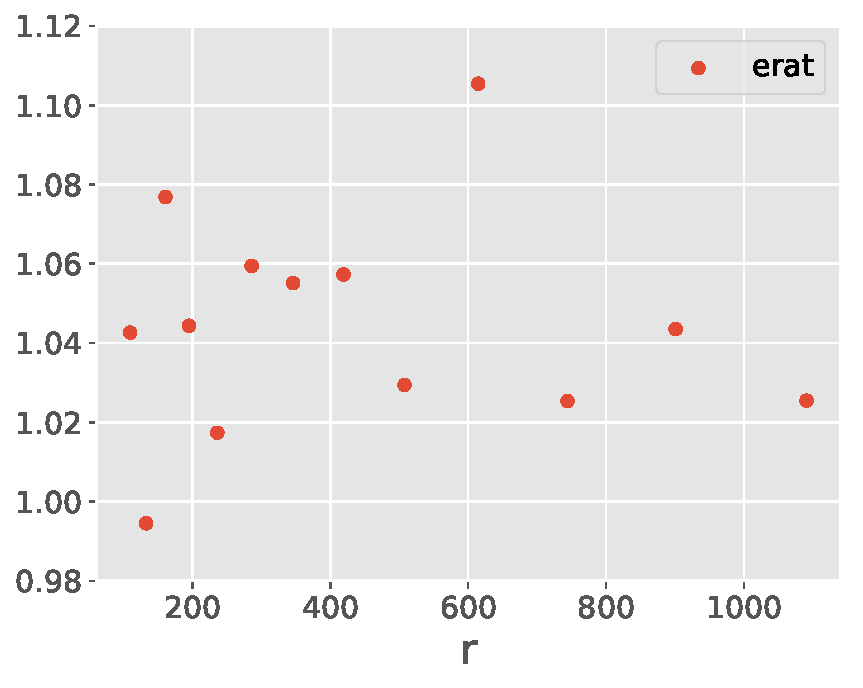
\includegraphics[width=0.48\textwidth,height=0.5\textwidth]{erat}
    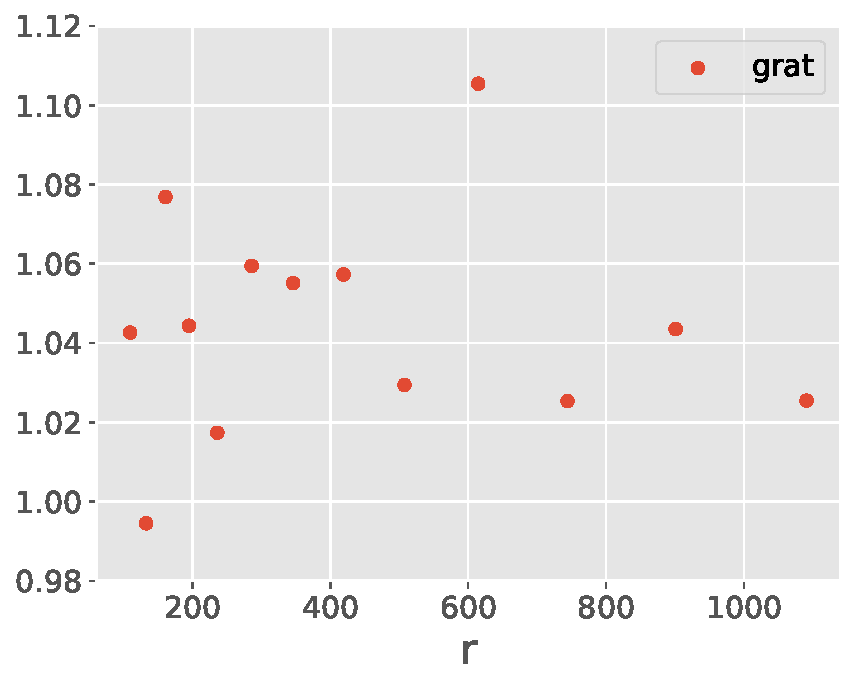
\includegraphics[width=0.48\textwidth,height=0.5\textwidth]{grat}
    \caption{Ellipticites and Shears Ratio (chromatic/monochromatic) }
\end{figure}
\section{Timeline}
I intend to complete all elements of this project within two years.
An outline of the projected time line is presented in the table below.
The dates and activities displayed are subject to change should
unforeseen and interesting developments occur during the projects that
may require special attention and time.
\begin{table}[h]
\caption{Time-line}
\vspace{5mm}
\centering
        \begin{tabular}{|c|c|c|}
            \hline
            Start&Finish&Activity\\
            \hline
            Aug. 2014& March 2017 &  Working on galaxy simulating software Jedisim \\
            \hline
            April 2017 & Jan. 2018 &  Release of Jedisim version 1.0 \\
            \hline
            Sep. 2018 & March 2019 & Integrating Jedisim with LSST pipelines \\
            \hline
            March 2019 & Aug. 2019& Writing and defending the Ph.D. dissertation   \\
            \hline
            \end{tabular}
\end{table}



%
%
%#******************************************************************************
%#==============================================================================
%#               Bibliography and End Document
%#==============================================================================
%#******************************************************************************
%
%
\newpage
\bibliographystyle{plainnat}
\bibliography{bib/prospectus}
\end{document}
